% IMPORTANT
 
% Install tex distribution
% https://www.latex-project.org/get/
% With Windows, install MikTeX
 
% in RStudio, install.packages("knitR")
% also, install all packages that appear in first code chunk in this file, i.e. in the one that looks like this
% <<LoadingPackages, include=FALSE>>=
% library(knitr)
% library(xtable)
% library(dplyr)
% library(stargazer)
% library(cowplot)
% @

% Go to Tools/Global Options/Sweave
% Select Weave Rnw files using: knitr
% Select Typeset LaTeX into PDF using: pdfLaTeX
 
% Use button "Compile PDF" to knit the Rnw file to a tex file and compile the tex file to a pdf file.

% Always install all packages that you're asked to after having pressed "Compile PDF".
 
% If there is no error while knitting from Rnw to tex, but an error while compiling from tex to pdf, have a look at the pdf file. It might still have worked.










% Load graphicx package in your document's preamble
% Gandrud (2016), p.192

% turn page 90 degrees with lscape Gandrud (2016), p.185

% Create clickable hyperlinks with hyperref package, Gandrud (2016), p. 218

% Use natbib package for bibliography formatting, authoryear for Harvard style , Gandrud (2016), p. 227
% commands to change what information is included in the parentheses, Gandrud (2016), p. 228, table 11.2

% Using saveRDS and readRDS, following 
% https://csgillespie.github.io/efficientR/efficient-inputoutput.html#efficient-data-export-.rdata-or-.rds

% working with knitR and LaTeX
% https://kbroman.org/knitr_knutshell/pages/latex.html
% Command line
% R -e 'library(knitr);knit("knitr_example.Rnw")'

% rotate tables in knitr
% https://stackoverflow.com/questions/21840878/rotate-a-table-from-r-markdown-in-pdf
% in particular stargazer tables
% https://stackoverflow.com/questions/31169845/rotate-stargazer-table-in-knitr/34292292#34292292

% Create list of packages used, Gandrud (2016), p 218/219

\documentclass[12pt, a4paper]{article}\usepackage[]{graphicx}\usepackage[]{color}
% maxwidth is the original width if it is less than linewidth
% otherwise use linewidth (to make sure the graphics do not exceed the margin)
\makeatletter
\def\maxwidth{ %
  \ifdim\Gin@nat@width>\linewidth
    \linewidth
  \else
    \Gin@nat@width
  \fi
}
\makeatother

\definecolor{fgcolor}{rgb}{0.345, 0.345, 0.345}
\newcommand{\hlnum}[1]{\textcolor[rgb]{0.686,0.059,0.569}{#1}}%
\newcommand{\hlstr}[1]{\textcolor[rgb]{0.192,0.494,0.8}{#1}}%
\newcommand{\hlcom}[1]{\textcolor[rgb]{0.678,0.584,0.686}{\textit{#1}}}%
\newcommand{\hlopt}[1]{\textcolor[rgb]{0,0,0}{#1}}%
\newcommand{\hlstd}[1]{\textcolor[rgb]{0.345,0.345,0.345}{#1}}%
\newcommand{\hlkwa}[1]{\textcolor[rgb]{0.161,0.373,0.58}{\textbf{#1}}}%
\newcommand{\hlkwb}[1]{\textcolor[rgb]{0.69,0.353,0.396}{#1}}%
\newcommand{\hlkwc}[1]{\textcolor[rgb]{0.333,0.667,0.333}{#1}}%
\newcommand{\hlkwd}[1]{\textcolor[rgb]{0.737,0.353,0.396}{\textbf{#1}}}%
\let\hlipl\hlkwb

\usepackage{framed}
\makeatletter
\newenvironment{kframe}{%
 \def\at@end@of@kframe{}%
 \ifinner\ifhmode%
  \def\at@end@of@kframe{\end{minipage}}%
  \begin{minipage}{\columnwidth}%
 \fi\fi%
 \def\FrameCommand##1{\hskip\@totalleftmargin \hskip-\fboxsep
 \colorbox{shadecolor}{##1}\hskip-\fboxsep
     % There is no \\@totalrightmargin, so:
     \hskip-\linewidth \hskip-\@totalleftmargin \hskip\columnwidth}%
 \MakeFramed {\advance\hsize-\width
   \@totalleftmargin\z@ \linewidth\hsize
   \@setminipage}}%
 {\par\unskip\endMakeFramed%
 \at@end@of@kframe}
\makeatother

\definecolor{shadecolor}{rgb}{.97, .97, .97}
\definecolor{messagecolor}{rgb}{0, 0, 0}
\definecolor{warningcolor}{rgb}{1, 0, 1}
\definecolor{errorcolor}{rgb}{1, 0, 0}
\newenvironment{knitrout}{}{} % an empty environment to be redefined in TeX

\usepackage{alltt}
\usepackage{lscape}
\usepackage{graphicx}
\usepackage[utf8]{inputenc}
\usepackage[backend=biber, bibstyle=apa, citestyle=authoryear]{biblatex}
\usepackage{floatrow}
\usepackage[hidelinks]{hyperref}
\usepackage{rotating}
% \usepackage[authoryear]{natbib}
% \bibliographystyle{apalike}
\usepackage{mathtools}
\usepackage[onehalfspacing]{setspace}
\usepackage[left = 72 pt, right = 72 pt]{geometry}

\addbibresource{references.bib}





\title{Effects of CHILDREN's programs}
\author{Laura Huber, Laura Jepsen, Jonathan Kirschner, Rafael Schütz, Yannick Zurl}
\date{27th February 2020}
\IfFileExists{upquote.sty}{\usepackage{upquote}}{}
\begin{document}

\begin{titlepage}
\maketitle
\end{titlepage}

\tableofcontents
\listoftables
\listoffigures

% To have an unnumbered section, place an sterisk in it like this \*{Unnumbered Section}
\section{Outline}
Descriptive statistics\\
dynamics of\\ 
(- number of organizations)\\
(- number of beneficiaries)\\
- selected ordinal outcomes, stacked\\
- real total subsidy\\
- real median subsidy per institution\\
- real median subsidy per beneficiary\\
(- which variables have largest variance; also relevant for variable selection)\\

Regressions\\

Questions:\\
effect of\\
- healthy meals (DGE criterion) on healthy characteristics\\
- real meals subsidy on number of meals\\
- real trips subsidy on number of trips\\
- real meals subsidy on self-worth and day-to-day skills\\
- real trips subsidy on self-worth and day-to-day skills\\

Methods:\\
- simple, metric\\
- standardized, metric\\
- cumulative logit\\
- with control variables\\
(- without outliers)\\
(- imputed data)\\

Diff in Diff\\

Outlook for CHILDREN/variable selection\\
- double selection \\
- partition analysis\\
(- correlation matrix)\\
(- factor analysis)\\
- general tips\\

\section{Introduction}

CHILDREN's aims for data analysis\\ 
CHILDREN supports organizations working with children and youth across Germany (in German: Einrichtungen der offenen Kinder- und Jugendarbeit) across Germany. We call them organizations in the following. They apply to CHILDREN for yearly grants. If approved, they are supposed to use them for specific purposes defined by CHILDREN. CHILDREN provided us with data from two of its flagship programs: Mittagstisch (we refer to this as Meals program) and Entdeckerfonds (Trips program). The organizations use money from the Meals program to finance meals, from breakfast to dinner, that they sell at concessionary prices to the children and youth that visit them. In the following, we call these children and youth who ultimately profit from CHILDREN's grants beneficiaries. The organizations also use money from the Trips program to make trips to nearby places usually unknown to the beneficiaries.  
Unless otherwise specified, we consider all variables to be metric, even if they are ordinal. 

\section{Summary Statistics}

% <<results='asis', echo=FALSE>>=
% tableCyclicDisp = readRDS("./Analysis/CyclicDisp.Rds")
% colnames(tableCyclicDisp) <- c("Lead in years", "All", "p-value", "Non-Durables", "p-value", "Durables", "p-value")
% tableCyclicDisp <- xtable(tableCyclicDisp, caption = "Cyclicality of productivity dispersion", digits = c(0, 0, 3, 2, 3, 2, 3, 2))
% print(tableCyclicDisp, include.rownames = FALSE)
% @

% latex table generated in R 3.6.2 by xtable 1.8-4 package
% Mon Feb 24 11:03:13 2020
\begin{table}[ht]
\centering
\begin{tabular}{mmmmm}
  \hline
Year & Beneficiaries, Meals & Beneficiaries, Trips & Organizations, Meals & Organizations, Trips \\ 
  \hline
2011 & 3748.0 &  & 52 &  \\ 
  2012 & 3556.0 & 2803.0 & 51 & 44 \\ 
  2013 & 4015.0 & 2823.0 & 55 & 42 \\ 
  2014 & 4685.0 & 2752.0 & 55 & 43 \\ 
  2015 & 5857.0 & 3823.0 & 55 & 49 \\ 
  2016 & 3075.0 & 3819.0 & 59 & 48 \\ 
  2017 & 4895.0 & 4150.0 & 64 & 48 \\ 
  2018 & 5102.5 & 6911.0 & 68 & 49 \\ 
   \hline
\end{tabular}
\caption{Summary Statistics} 
\end{table}

% look up official names of price indices in English 
At the beginning of the time series in 2011, they supported in x institutions. In 2018, this number had increased to y. In this section, we give an overview of the dynamics of CHILDREN's two flagship programs. We focus on the number of estimated ultimate beneficiaries, median total subsidy, median subsidy per institution, and median subsidy per beneficiary. We also look at selected outcomes, i.e. those related to health as well as self-worth and day-to-day skills. We have converted all nominal monetary variables into 2015 euros, using price indices from the Federal Statistical Office of Germany (Statistisches Bundesamt). We deflate (requested) grants as well as organizations' total expenses for the Meals program  with the price index related to food and non-alcoholic beverages (in German: Nahrungsmittel und alkoholfreie Getränke) and (requested) grants towards the Trips program with the price index for leisure, entertainment, and culture (in German: Freizeit, Unterhaltung und Kultur). These are only available after logging in on DESTATIS. The organizations also gave information about their total yearly budget. We inflate this with the general price index.    

\begin{figure}
  \caption{Yearly dynamics of total grants in Meals program}
  \label{totalGrantsDyn}

\begin{knitrout}
\definecolor{shadecolor}{rgb}{0.969, 0.969, 0.969}\color{fgcolor}\begin{kframe}
\begin{verbatim}
## NULL
\end{verbatim}
\end{kframe}
\end{knitrout}

\floatfoot{This graph shows the development of the sum of all grants in the Meals program. We have deflated the values to 2015 euros using the price index related to food and non-alcoholic beverages(in German: Nahrungsmittel und alkoholfreie Getränke) provided by the Federal Statistical Office of Germany (Statistisches Bundesamt).}
\end{figure}




Examples\\

Equation\\

\begin{equation}
\label{ModelProdu}
\ln y_{it} = \beta_0 + \beta_k \ln k_{it-1} + \beta_n \ln n_{it} + \beta_m \ln m_{it} + \beta_t D_t + \beta_i D_i + \epsilon_{it}
\end{equation}

List\\

\begin{itemize}
  \item{The firm is not incorporated in the U.S. (FIC is not equal to USA.)}
  \item{The company is from the financial or utilities sector. This is the case when the SIC code lies between 4900 and 4999 or between 6000 and 6999.}
  \item{A firm's acquisitions are larger than five percent of the value of its total assets. This is the case when AQC over AT is larger than 0.05.} 
\end{itemize}


Figure\\

\begin{figure}
  \caption{Dispersion in productivity levels}
  \label{LineDisp}

\begin{knitrout}
\definecolor{shadecolor}{rgb}{0.969, 0.969, 0.969}\color{fgcolor}

{\centering 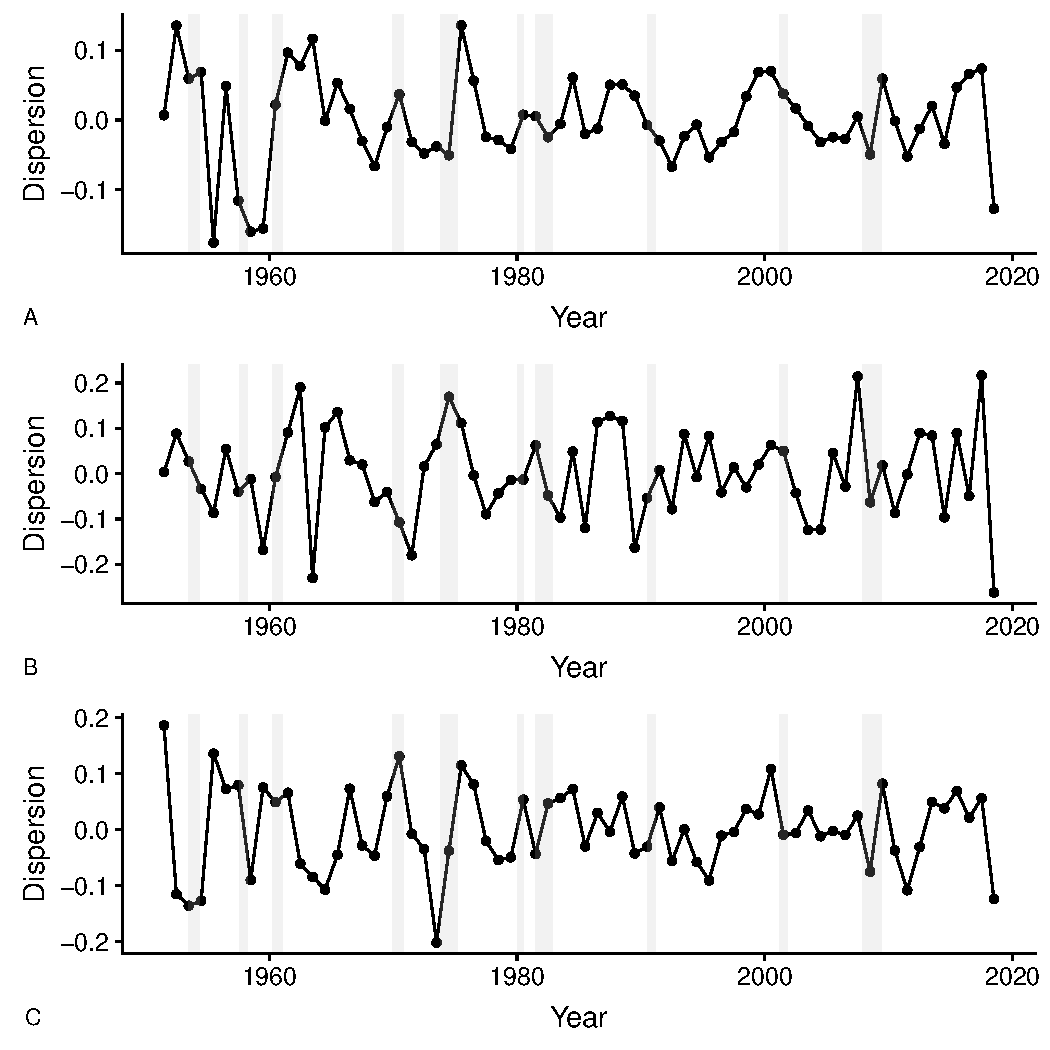
\includegraphics[width=0.8\textwidth]{figure/unnamed-chunk-2-1} 

}



\end{knitrout}

\floatfoot{Note: Time series plots of approximate deviations of the three annual dispersion measures from their trends in percent. A shows the full sample, B the non-durable manufacturing sector, and C the durable manufacturing sector. After taking the natural logarithm of the dispersion measures defined in equation 1, I have isolated their cyclical components with an HP-100 filter. The shaded bars represent recessions as defined by the NBER. The year ticks refer to January 1. The dispersion measures take as their date the middle of the year, July 2. Compare Kehrig (2015), Figure 1.}
\end{figure}

\section{The effect of the "Entdeckerfonds" on the beneficiaries of the program}

How do children benefit from visiting social institutions that CHILDREN supports financially? So far this question could not be empirically validated. Hence, one of the biggest challenges was determining a possible solution for measuring causal effects of the programs on the beneficiaries. During the first meeting with CHILDREN, Wiltrud de Haan presented relevant information that CHILDREN supports all organizations with the Mittagstisch program. However, not all organizations do receive addtitional funding to provide the Entdeckerfonds program. This fact could be used for applying an empirical approach which determines causal effects of the Entdeckerfonds program by comparing a treatment with a control group. The aim of this analysis is to show that the trips provided by Entdeckerfonds program funding have a positive effect on selfworth and everyday expertise of the participating children. 


Empirical Approach\\

The baseline of the empirical approach is the determination of the treatment and control group. Using the data provided by children we specify the treatment group as all organizations that receive funding for both the Entdeckerfonds and the Mittagstisch program. On the other hand, the control group represents all organizations that do not receive funding from CHILDREN to provide the Entdeckerfonds.

Determining the treatment and control group this way, however, was a problem.

THerefore we used the cleaned data set and only determined the control group - all organizations that have no values/answers for the questions of the Entdeckerfonds. We assume that these organizations did not receive the funding for the Entdeckerfonds and therefore are the control group in our analysis. All organizations that gave answers to at least one question of the survey part regarding the entdeckerfonds are considered the treatment group. 
Our analysis is based on this very strong definition of the treatment and control group.

Because we do not have data for the entdeckerfonds survey for the control group as this group is not observed we use the answers of the mittagstisch survey for our analysis. THerefore our possible dependent variables are limited as most of the questions are specific to the meals program. 

As the dataset does not include the variables for the Entdeckerfonds survey for the control group, the potential outcomes regarding the Entdeckerfonds are not observed. Therefore we have to use the survey answers from the Mittagstisch survey.

Generally our data set contains variables from the years 2011 until 2018. 

The constellation of the treatment and control group varies from year to year. 
Assumption: erhalten der treatment gleichbedeutend wie ein verlust

Possible variables as dependent variables
how we determined that:
The used variables should not be specific to the mittagstisch but more general and should also apply to the context of the Entdeckerfonds
possible variables selfworth, day to day skills
used these variables because these variables could be influenced both by the mittagstisch and entdeckerfonds and are not specific to the entdeckerfonds

looked at the general trends of these two variables with the difference of the treatment and control group to look at whether our idea makes sense

linear regression just to look at whether there are effects

add controls and fixed effects time and id fixedeffects --> explain why (id: specific effects of being in Bayern for example or the subsidy amount)
how fixed effects are implemented

which control variables we use
how we determined which controls





Ende??
the dataset does not allow a channel analysis but these could be possible channels that might explain the effects we find


% Table created by stargazer v.5.2.2 by Marek Hlavac, Harvard University. E-mail: hlavac at fas.harvard.edu
% Date and time: Mo, Feb 24, 2020 - 11:03:14
% Requires LaTeX packages: dcolumn rotating 
\begin{sidewaystable}[!htbp] \centering 
  \caption{Regression Results} 
  \label{} 
\begin{tabular}{@{\extracolsep{5pt}}lD{.}{.}{-3} D{.}{.}{-3} D{.}{.}{-3} D{.}{.}{-3} } 
\\[-1.8ex]\hline 
\hline \\[-1.8ex] 
 & \multicolumn{4}{c}{\textit{Dependent variable:}} \\ 
\cline{2-5} 
\\[-1.8ex] & \multicolumn{4}{c}{selfworth} \\ 
\\[-1.8ex] & \multicolumn{1}{c}{(1)} & \multicolumn{1}{c}{(2)} & \multicolumn{1}{c}{(3)} & \multicolumn{1}{c}{(4)}\\ 
\hline \\[-1.8ex] 
 Constant & 2.796^{***} & 2.870^{***} & 2.774^{***} & 2.847^{***} \\ 
  & (0.065) & (0.095) & (0.092) & (0.107) \\ 
  & & & & \\ 
 treatEF & 0.249^{***} & 0.320^{***} & 0.253^{***} & 0.333^{***} \\ 
  & (0.074) & (0.097) & (0.075) & (0.100) \\ 
  & & & & \\ 
\hline \\[-1.8ex] 
ID fixed effects & No & No & Yes & Yes \\ 
Time fixed effects & No & Yes & No & Yes \\ 
Observations & \multicolumn{1}{c}{430} & \multicolumn{1}{c}{430} & \multicolumn{1}{c}{430} & \multicolumn{1}{c}{430} \\ 
R$^{2}$ & \multicolumn{1}{c}{0.026} & \multicolumn{1}{c}{0.035} & \multicolumn{1}{c}{0.026} & \multicolumn{1}{c}{0.036} \\ 
Adjusted R$^{2}$ & \multicolumn{1}{c}{0.024} & \multicolumn{1}{c}{0.017} & \multicolumn{1}{c}{0.022} & \multicolumn{1}{c}{0.015} \\ 
Residual Std. Error & \multicolumn{1}{c}{0.642 (df = 428)} & \multicolumn{1}{c}{0.644 (df = 421)} & \multicolumn{1}{c}{0.642 (df = 427)} & \multicolumn{1}{c}{0.645 (df = 420)} \\ 
F Statistic & \multicolumn{1}{c}{11.417$^{***}$ (df = 1; 428)} & \multicolumn{1}{c}{1.916$^{*}$ (df = 8; 421)} & \multicolumn{1}{c}{5.752$^{***}$ (df = 2; 427)} & \multicolumn{1}{c}{1.724$^{*}$ (df = 9; 420)} \\ 
\hline 
\hline \\[-1.8ex] 
\textit{Note:}  & \multicolumn{4}{r}{$^{*}$p$<$0.1; $^{**}$p$<$0.05; $^{***}$p$<$0.01} \\ 
\end{tabular} 
\end{sidewaystable} 



% table1_selfworth <- stargazer(lm1_selfworth,
%                     lm2_selfworth,
%                     lm3_selfworth,
%                     lm4_selfworth,
%           title = "Regression Results",
%           order = c('Constant', 'treatEF'),
%           omit = c('id104','id105','id106','id108','id109','id111','id112','id113','id114','id118','id122',
%                    'id123','id124','id125','id130','id131','id132','id133','id136','id137','id139','id141',
%                    'id142','id165','id186','id187','id188','id189','id190','id191','id192','id193','id194',
%                    'id209','id213','id214','id215','id216','id217','id218','id219','id220','id221','id226',
%                    'id233','id249','id255','id269','id270','id281','id282','id403','id404','id417','id418',
%                    'id437','id482','id483','id599','id600','id601','id602','id623','id684','id685','id686',
%                    'id687','dummy_2012','dummy_2013','dummy_2014','dummy_2015','dummy_2016','dummy_2017',
%                    'dummy_2018', 'id'
%                   ),
%           add.lines = list(c("ID fixed effects", 'No', 'No', 'Yes', 'Yes'),
%                            c('Time fixed effects', 'No', 'Yes', 'No', 'Yes')),
%           align = TRUE)

% \begin{table}[!htbp] \centering 
%   \caption{Regression Results} 
%   \label{} 
% \begin{tabular}{@{\extracolsep{5pt}}lD{.}{.}{-3} D{.}{.}{-3} D{.}{.}{-3} D{.}{.}{-3} } 
% \\[-1.8ex]\hline 
% \hline \\[-1.8ex] 
%  & \multicolumn{4}{c}{\textit{Dependent variable:}} \\ 
% \cline{2-5} 
% \\[-1.8ex] & \multicolumn{4}{c}{selfworth} \\ 
% \\[-1.8ex] & \multicolumn{1}{c}{(1)} & \multicolumn{1}{c}{(2)} & \multicolumn{1}{c}{(3)} & \multicolumn{1}{c}{(4)}\\ 
% \hline \\[-1.8ex] 
%  Constant & 2.796^{***} & 2.870^{***} & 2.774^{***} & 2.847^{***} \\ 
%   & (0.065) & (0.095) & (0.092) & (0.107) \\ 
%   & & & & \\ 
%  treatEF & 0.249^{***} & 0.320^{***} & 0.253^{***} & 0.333^{***} \\ 
%   & (0.074) & (0.097) & (0.075) & (0.100) \\ 
%   & & & & \\ 
% \hline \\[-1.8ex] 
% ID fixed effects & No & No & Yes & Yes \\ 
% Time fixed effects & No & Yes & No & Yes \\ 
% Observations & \multicolumn{1}{c}{430} & \multicolumn{1}{c}{430} & \multicolumn{1}{c}{430} & \multicolumn{1}{c}{430} \\ 
% R$^{2}$ & \multicolumn{1}{c}{0.026} & \multicolumn{1}{c}{0.035} & \multicolumn{1}{c}{0.026} & \multicolumn{1}{c}{0.036} \\ 
% Adjusted R$^{2}$ & \multicolumn{1}{c}{0.024} & \multicolumn{1}{c}{0.017} & \multicolumn{1}{c}{0.022} & \multicolumn{1}{c}{0.015} \\ 
% Residual Std. Error & \multicolumn{1}{c}{0.642 (df = 428)} & \multicolumn{1}{c}{0.644 (df = 421)} & \multicolumn{1}{c}{0.642 (df = 427)} & \multicolumn{1}{c}{0.645 (df = 420)} \\ 
% F Statistic & \multicolumn{1}{c}{11.417$^{***}$ (df = 1; 428)} & \multicolumn{1}{c}{1.916$^{*}$ (df = 8; 421)} & \multicolumn{1}{c}{5.752$^{***}$ (df = 2; 427)} & \multicolumn{1}{c}{1.724$^{*}$ (df = 9; 420)} \\ 
% \hline 
% \hline \\[-1.8ex] 
% \textit{Note:}  & \multicolumn{4}{r}{$^{*}$p$<$0.1; $^{**}$p$<$0.05; $^{***}$p$<$0.01} \\ 
% \end{tabular} 
% \end{table}







\printbibliography
\end{document}
